\documentclass{beamer}
\usepackage[UTF8]{ctex}
\usepackage{lmodern}
\usepackage{bm}
\mode<presentation> {
	
	% The Beamer class comes with a number of default slide themes
	% which change the colors and layouts of slides. Below this is a list
	% of all the themes, uncomment each in turn to see what they look like.
	
	%\usetheme{default}
	%\usetheme{AnnArbor}
	%\usetheme{Antibes}
	%\usetheme{Bergen}
	%\usetheme{Berkeley}
	%\usetheme{Berlin}
	%\usetheme{Boadilla}
	%\usetheme{CambridgeUS}
	\usetheme{Copenhagen}
	%\usetheme{Darmstadt}
	%\usetheme{Dresden}
	%\usetheme{Frankfurt}
	%\usetheme{Goettingen}
	%\usetheme{Hannover}
	%\usetheme{Ilmenau}
	%\usetheme{JuanLesPins}
	%\usetheme{Luebeck}
	%\usetheme{Madrid}
	%\usetheme{Malmoe}
	%\usetheme{Marburg}
	%\usetheme{Montpellier}
	%\usetheme{PaloAlto}
	%\usetheme{Pittsburgh}
	%\usetheme{Rochester}
	%\usetheme{Singapore}
	%\usetheme{Szeged}
	%\usetheme{Warsaw}
	
	% As well as themes, the Beamer class has a number of color themes
	% for any slide theme. Uncomment each of these in turn to see how it
	% changes the colors of your current slide theme.
	
	%\usecolortheme{albatross}
	%\usecolortheme{beaver}
	%\usecolortheme{beetle}
	%\usecolortheme{crane}
	%\usecolortheme{dolphin}
	%\usecolortheme{dove}
	%\usecolortheme{fly}
	%\usecolortheme{lily}
	%\usecolortheme{orchid}
	%\usecolortheme{rose}
	%\usecolortheme{seagull}
	%\usecolortheme{seahorse}
	%\usecolortheme{whale}
	%\usecolortheme{wolverine}
	
	%\setbeamertemplate{footline} % To remove the footer line in all slides uncomment this line
	%\setbeamertemplate{footline}[page number] % To replace the footer line in all slides with a simple slide count uncomment this line
	
	%\setbeamertemplate{navigation symbols}{} % To remove the navigation symbols from the bottom of all slides uncomment this line
}

\usepackage{graphicx} % Allows including images
\usepackage{booktabs} % Allows the use of \toprule, \midrule and \bottomrule in tables 

\usepackage[T1]{fontenc}
\usepackage[utf8]{inputenc}
\setbeamertemplate{caption}[numbered]
\newcommand{\C}{\mathbb{C}}
\newcommand{\R}{\mathbb{R}}
\newcommand{\Q}{\mathbb{Q}}
\newcommand{\Z}{\mathbb{Z}}
\newcommand{\N}{\mathbb{N}}
\newcommand{\p}{\mathbb{P}}
\newcommand{\E}{\mathbb{E}}
\newcommand{\new}[1]{\textcolor{red}{#1}}
\usepackage{graphicx}
\usepackage{amssymb}
\usepackage{setspace}
\usepackage[toc,page]{appendix}
\usepackage{epstopdf}
\usepackage{latexsym}
\usepackage{amstext}
\usepackage{lmodern}
\usepackage{amsmath}
\usepackage{bbm}
\usepackage{amsfonts}
\usepackage{url}
\usepackage{bm}
\usepackage{mathrsfs}
\usepackage{mathtools}
\usepackage{float}
%\usepackage{hyperref} give reference hyperlink 
%\usepackage{setspace}
\usepackage{indentfirst}
\usepackage{multirow}
\usepackage{color}
\usepackage{mathtools}
% packages from template
\usepackage{amsmath,amsthm,amssymb,amsfonts}
\usepackage[width=.9\textwidth]{caption}
\usepackage{mathrsfs}
\usepackage{graphicx}
\newcommand{\indep}{\rotatebox[origin=c]{90}{$\models$}}
%\usepackage{textgreek}
\usepackage{bbold}
\usepackage{subcaption}
\usepackage{natbib}
\usepackage{verbatim}
\usepackage{soul}
\usepackage[utf8]{inputenc}
%\usepackage[algo2e,ruled,vlined]{algorithm2e} 
%\usepackage{fancyvrb}


\newtheorem{proposition}[theorem]{Proposition}

\newcommand{\M}{\boldsymbol{M}}
\newcommand{\rank}{\mathrm{rank}}
\newcommand{\rep}{\mathrm{rep}}
\newcommand{\PR}{\text{Pr}}
\newcommand{\pkg}[1]{{\fontseries{b}\selectfont #1}}
%\newcommand\norm[1]{\left\lVert#1\right\rVert}
\newcommand{\bs}[1]{\pmb{#1}}
\newcommand{\mb}[1]{\boldsymbol{#1}}
\DeclareMathOperator*{\argmin}{arg\,min}
\DeclarePairedDelimiter{\ceil}{\lceil}{\rceil}
\DeclarePairedDelimiterX{\norm}[1]{\lVert}{\rVert}{#1}
\allowdisplaybreaks
%=============================================================================
% prelude
%=============================================================================
\def\mathLarge#1{\mbox{\LARGE $#1$}}
\usepackage{soul}


\title[]{随机事件与概率}
\author[概率统计]{张宏达}
\institute{Nanjing University}
\date{}

\begin{document}
	\begin{frame}
		\titlepage
	\end{frame}
	\begin{frame}
		\frametitle{联系方式}
		微信群:
		\begin{figure}[H]
			\centering
			
\includegraphics[scale=0.13]{figures/概率统计05.png}
		\end{figure}
	Email:hongdazhang@nju.edu.cn
	\end{frame}
	
	\begin{frame}
		\frametitle{课程说明}
		\begin{itemize}
			\item 教学内容:教材第1-8章内容。其中第3章第4节条件分布为选讲。
			\item 成绩构成: 作业20\%,期中考试30\%,期末考试50\%。
			\item 考试时间:期中考试一般在第11周,涵盖前4章内容。
			\item 消息发布:课下主要在微信群内发布消息以及布置作业。
			\item 交作业:上课前放在讲台桌上。
		\end{itemize}
	\end{frame}
	
	\begin{frame}
		\frametitle{主要内容}
		\begin{itemize}
			\item 随机事件及其运算
			\item 事件的概率与性质
			\item 等可能事件
			\item 几何概率
			\item 条件概率
			\item 独立性
			\item 独立重复实验
		\end{itemize}
	\end{frame}
	\begin{frame}
		\frametitle{随机事件及其运算}
		\textbf{随机试验}是指对随机现象对一次观测,用$E$表示,其具有如下特点
		\begin{itemize}
			\item 在相同条件下试验可重复进行。
			\item 每次试验有多种结果,并试验之前可知道试验所有可能结果。
			\item 每次试验会随机出现一个结果。
		\end{itemize}
		随机试验$E$可能出现的所有结果的集合被称为$\textbf{样本空间}$,用$\Omega$表示。每一个可能的结果被称为$\textbf{基本事件}$或$\textbf{样本点}$,记为$e$。
		
		\vspace{1cm}
		
		示例1 某班级共10人,我们关心某天迟到人数。
		
		$E1$:观察此班级当天迟到人数。
		$\Omega_1$ = $\{0, 1, 2, \dots, 10\}$。这里共有11个样本点。
	\end{frame}
	
	\begin{frame}
		\textbf{随机事件}(简称\textbf{事件})是样本空间的子集。
		
		根据示例1可以定义随机事件$A=\{1, 2\}, B = \{0, 1, 2\}$。
		
		随机事件的发生:只要随机事件中包含的任何样本点发生,则称该随机事件发生。
		
		\textbf{必然事件}:样本空间$\Omega$。必然发生的事件。
		
		\textbf{不可能事件}:空集$\phi$。必然不发生的事件。
		
		事件间的关系:
		\begin{itemize}
			\item 包含关系。如果事件$A$发生必然导致事件$B$发生,则称事件$B$包含事件$A$,记为$B \supset A$。仍以示例1为例。有1人或2人迟到必然导致有0,1,或者2人迟到。
			\item 互不相容关系。事件不可能同时发生则称事件互不相容(或互斥)。此时事件没有公共的样本点。定义新事件$C = \{3, 4\}, D = \{2, 3, 4\}$。则事件$A$,$C$互不相容,而$A$,$D$有交集。
			\item 相等关系。两个事件相等时其包含的样本点完全相同。比如事件B与事件$F=\{\text{至多两人迟到}\}$。
		\end{itemize}
	\end{frame}
	\begin{frame}
		事件的运算
		\begin{itemize}
			\item 事件的并。事件$A$,$B$至少发生一个所构成的事件称为$A$与$B$的并,记为$A\cup B$。其中的样本点为各自事件样本点的并集。
			
			例如定义随机试验:甲乙各自射击记录命中情况。$A = \{\text{甲命中}\}, B = \{\text{乙命中}\}$。则$A\cup B = \{\text{甲或者乙命中}\}$。
			
			推广:对于多个事件$A_1, A_2, \dots, A_n$。它们的并记为$\cup_{i = 1}^{n}A_i$,表示这些事件中至少有一个发生。
			\item 事件的交。如果事件$A$, $B$同时发生,记为$A\cap B$,称为$A$与$B$的交。
			
			推广:事件$A_1, A_2, \dots, A_n$同时发生称为$A_1, A_2, \dots, A_n$的交,记为$\cap_{i = 1}^{n}A_i$,或$A_1 A_2 A_3 \cdots A_n$。
			\item 事件的差事件A发生而B不发生的事件称为A与B的差,记为$A-B$。
			\item 对立事件。A不发生的事件被称为A的对立事件,记为$\bar{A}$。
		\end{itemize}
	\end{frame}
	
	\begin{frame}
		例1.1 假设我们关心同学甲、乙是否来听课。$A = \{\text{甲来听课}\}$, $B = \{\text{乙来听课}\}$。则
		\begin{itemize}
			\item $A\cup B =$
			\item $A\cap B =$
			\item $A - B =$
			\item $\bar{A} =$
		\end{itemize}
		
%		事件本质上是集合所以遵循集合的运算律:
%		\begin{itemize}
%			\item 交换律:$A\cup B = B\cup A, A\cap B = B\cap A$。
%			\item 结合律:$(A\cup B)\cup C = A\cup (B \cup C), (A\cap B)\cap C = A\cap (B \cap C)$。
%			\item 分配率:$A \cup ( B \cap C) = (A\cup B)\cap (A \cup C)$, $A \cap ( B \cup C) = (A\cap B)\cup (A \cap C)$
%		\end{itemize}
	\end{frame}
	
	\begin{frame}
		例1.1 假设我们关心同学甲、乙是否来听课。$A = \{\text{甲来听课}\}$, $B = \{\text{乙来听课}\}$。则
		\begin{itemize}
			\item $A\cup B = \{\text{甲或者乙来听课}\}$。
			\item $A\cap B = \{\text{甲来听课并且乙来听课}\}$。
			\item $A - B = \{\text{甲来听课且乙不来听课}\}$。
			\item $\bar{A} = \{\text{甲不来听课}\}$
		\end{itemize}
		
		事件本质上是集合所以遵循集合的运算律:
		\begin{itemize}
			\item 交换律:$A\cup B = B\cup A, A\cap B = B\cap A$。
			\item 结合律:$(A\cup B)\cup C = A\cup (B \cup C), (A\cap B)\cap C = A\cap (B \cap C)$。
			\item 分配率:$A \cup ( B \cap C) = (A\cup B)\cap (A \cup C)$, $A \cap ( B \cup C) = (A\cap B)\cup (A \cap C)$
		\end{itemize}
	\end{frame}
	
	\begin{frame}
		\frametitle{事件的概率与性质}
		假设随机事件$A$在$n$次独立重复试验中出现$n_A$次,则
		\[
		f_n(A) = \frac{n_A}{n},
		\]
		被称为$A$发生的\textbf{频率}。
		
		示例2:重复投掷骰子100次,其中16次出现6点。则事件$A = \{\text{出现6点}\}$的频率$f_{100}(\{\text{出现6点}\}) = 16 / 100$.
		
		频率的性质:
		\begin{itemize}
			\item $0 \leq f_n(A) \leq 1$
			\item $f_n(\Omega) = 1$
			\item 如果事件$A_1, A_2, \dots, A_n$互不相容,则
			\[
			f_n(\cup_{i = 1}^{n}A_i) = \sum_{i = 1}^{n}f_n(A_i)
			\]
		\end{itemize}
		随着试验次数$n$的增加,频率趋近于的数值被称为\textbf{统计概率}。
	\end{frame}
	
	\begin{frame}
		定义1.1 设E是随机试验,$\Omega$为其样本空间。对于E中任意一个随机事件$A$,对应一个实数$P(A)$。如果集合函数$P(\cdot)$满足:
		\begin{itemize}
			\item 非负性: $P(A) \geq 0$
			\item 规范性: $P(\Omega) = 1$
			\item 可列可加性: 若$A_1, A_2, \dots$两两互不相容,则
			\[
			P(\cup_{i = 1}^{\infty}A_i) = \sum_{i = 1}^{\infty}P(A_i)
			\]
		\end{itemize}
		则称$P(A)$为事件$A$的概率。
		
		概率函数有如下性质:
		\begin{enumerate}
			\item $P(\phi) = 0$
			\item 若$A_1, A_2, \dots, A_n$两两互不相容,则
			\[
			P(\cup_{i = 1}^{n}A_i) = \sum_{i = 1}^{n}P(A_i)
			\]
		\end{enumerate}
	\end{frame}
	
	\begin{frame}
		\begin{enumerate}
			\setcounter{enumi}{2}
			\item 对于任意两个事件A和B,$P(A - B) = P(A) - P(A \cap B)$. (提示:$A - B = A - A \cap B$.)
			\item 对于任意两个事件A,B,有\textbf{加法定理}
			\[
			P(A \cup B) = P(A) + P(B) - P(A \cap B)
			\]
			(提示:$A \cup B = A + (B - A \cap B)$)
			\item 对任意事件A,$P(\bar{A}) = 1 - P(A)$. 
		\end{enumerate}
	\end{frame}
	
	\begin{frame}
		\frametitle{等可能概型(古典概型)}
		等可能概型有如下特点:
		\begin{itemize}
			\item 样本空间样本点个数有限。
			\item 样本空间中每个样本点发生的概率相同。
		\end{itemize}
		假设随机试验$E$为等可能概型,并且样本空间有n个样本点。如果事件A含有m个样本点,则事件A的概率
		\[
		P(A) = \frac{m}{n} = \frac{\text{A中包含样本点数}}{\text{样本点总数}}
		\]
	\end{frame}
	
	\begin{frame}
		例1.3 一盒元件有45个正品,5个次品。从中任取5个,则以下事件概率是多少
		\begin{enumerate}
			\item A:恰好有3个正品。
			\item B:至多有2个次品。
		\end{enumerate}
%		\begin{enumerate}
%			\item 样本点总数为从50个元件中取出5个的所有可能取法(忽略次序)即$n = C_{50}^{5}$。
%			事件A的样本点数为$C_{45}^3 \times C_{5}^2$.这样
%			\[
%			P(A) = \frac{C_{45}^3 \times C_{5}^2}{C_{50}^{5}}
%			\]
%			\item $B = \{\text{至多有2个次品}\} = \{\text{有5个正品}\} \cup \{\text{有4个正品和1个次品}\} \cup \{\text{有3个正品和2个次品}\}$
%			\[
%			P(B) = \frac{C_{45}^5 \times C_{5}^{0} + C_{45}^4 \times C_{5}^{1} + C_{45}^{3} \times C_{5}^{2} }{C_{50}^5}
%			\]
%		\end{enumerate}
	\end{frame}
	
	\begin{frame}
		例1.3 一盒元件有45个正品,5个次品。从中任取5个,则以下事件概率是多少
		\begin{enumerate}
			\item A:恰好有3个正品。
			\item B:至多有2个次品。
		\end{enumerate}
		\begin{enumerate}
			\item 样本点总数为从50个元件中取出5个的所有可能取法(忽略次序)即$n = C_{50}^{5}$。
			事件A的样本点数为$C_{45}^3 \times C_{5}^2$.这样
			\[
			P(A) = \frac{C_{45}^3 \times C_{5}^2}{C_{50}^{5}}
			\]
			\item $B = \{\text{至多有2个次品}\} = \{\text{有5个正品}\} \cup \{\text{有4个正品和1个次品}\} \cup \{\text{有3个正品和2个次品}\}$
			\[
			P(B) = \frac{C_{45}^5 \times C_{5}^{0} + C_{45}^4 \times C_{5}^{1} + C_{45}^{3} \times C_{5}^{2} }{C_{50}^5}
			\]
		\end{enumerate}
	\end{frame}
	
		\begin{frame}
		例1.5 N件产品,含有M件次品,其余为正品。按照\textbf{不放回}和\textbf{有放回}两种方式从中取出n件.分别计算恰有$k, k \leq M$件次品的概率。
		%		\begin{itemize}
			%			\item 不放回情况:
			%			
			%			样本点总数为$C_N^n$。取出$k$件次品可分解为两步:第一步从$M$件次品中取出$k$件,第二步从$N - M$件正品中取出$n - k$件。这样
			%			\[
			%			p = \frac{C_M^k C_{N - M}^{n - k}}{C_N^n}
			%			\]	
			%		\end{itemize}
	\end{frame}
	
	\begin{frame}
		例1.5 N件产品,含有M件次品,其余为正品。按照\textbf{不放回}和\textbf{有放回}两种方式从中取出n件.分别计算恰有$k, k \leq M$件次品的概率。
		\begin{itemize}
			\item 不放回情况:
			
			样本点总数为$C_N^n$。取出$k$件次品可分解为两步:第一步从$M$件次品中取出$k$件,第二步从$N - M$件正品中取出$n - k$件。这样
			\[
			p = \frac{C_M^k C_{N - M}^{n - k}}{C_N^n}
			\]	
		\end{itemize}
	\end{frame}
	
	\begin{frame}
		\begin{itemize}
			\item 有放回情况:
			
			有放回时公式$C_N^n$不再适用。则需要用基本都乘法原理考虑问题。并且此时需要考虑抽取顺序。
			
			每一次抽取时都有$N$种选择,则考虑抽取次序的情况下,抽取$n$次共有$N^n$中不同的方式。
			此时考虑抽取到$k$个次品的情况。首先确定第几次抽取到次品。这样的情况有$C_n^k$个。之后抽取过程中次品和正品的次序就确定了。然后在每个位置放入次品或正品。这样每个次品位置有$M$种不同的选择,每个正品位置有$N - M$个选择。如此抽出$k$个次品的情况有
			\[
			C_n^k M^k (N - M) ^ {n - k}
			\]
			由此可知
			\[
			p = \frac{C_n^k M^k (N - M) ^ {n - k}}{N^                                                                                                                                                                                                                                                                                                                                                                                                                                                                                                                                                                                                                                                                                                                                                                                                                                                                                                                                                                                                                                                                                                                                                                                                                                                                                                                                                                                                                                                                                                                                                                                                                                                                                                                                                                                                                                                                                                                                                                                                                                                                                                                                                                                                                                                                                                                                                                                                                                                                                                                                                                                                                                                                                                                                                                                                                                                                                                                                                                                                                                                                                                                                                                                                                                                                                                                                                                                                                                                                                                                                                                                                                                                                                                                                                                                                                                                                                                                                                                                                                                                                                                                                                                                                                                                                                                                                                                                                                                                            n}
			\]
		\end{itemize}
	\end{frame}
	
	\begin{frame}
		\frametitle{几何概率}
		定义 1.2 若随机试验的样本空间$\Omega$对应一个度量有限的几何空间$S$,且所有的基本事件与$S$内的点一一对应,则任一随机事件$A$对应$\Omega$中的某一子区域$D$。若事件$A$的概率只和其对应的度量成正比,与D的形状及D在S中位置无关.A发生的概率定义为
		\[
		P(A) = \frac{m(A)}{m(\Omega)} = \frac{A\text{对应区域D的度量}}{\Omega\text{对应区域S的度量}}
		\]
		这样的概率被称为几何概率。
	\end{frame}
	
	\begin{frame}
		例1.10 在$[0, 1]$区间任取两个数,求两数之和小于1且两数之积小于2/9的概率。
	\end{frame}
	
	\begin{frame}
		例1.10 在$[0, 1]$区间任取两个数,求两数之和小于1且两数之积小于2/9的概率。
		
		首先确定任取两数这个随机试验的样本空间为$[0, 1] \times [0, 1]$的正方形区域。
		
		然后确定事件$A = \{(x, y) | 0 \leq x + y \leq 1, 0 \leq xy \leq 2 / 9\}$
	\end{frame}
	
	\begin{frame}
		\begin{figure}[H]
			\centering
			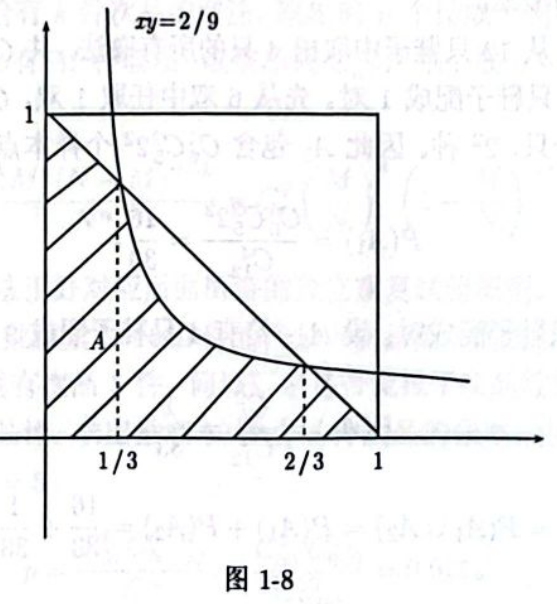
\includegraphics[scale = 0.4]{figures/figure1-8.png}
		\end{figure}
	\end{frame}
	
	\begin{frame}
		$\Omega$对应的面积为1。
		
		$A$对应的面积为图中阴影部分:
		\[
		1 / 2 - \int_{1 / 3}^{2 / 3}[(1 - x) - \frac{2}{9x}]dx = 1 / 3 + 2 / 9 \ln 2
		\]
		由此
		\[
		P(A) = \frac{m(A)}{m(\Omega)} = 1 / 3 + 2 / 9 \ln 2
		\]
	\end{frame}
	
	\begin{frame}
		例 1.11 甲乙两人约定8点到9点之间随机到达某地会面,先到者等待15分钟,过时不候。求两人能会面的概率。
		
	\end{frame}
	
	\begin{frame}
		例 1.11 甲乙两人约定8点到9点之间随机到达某地会面,先到者等待15分钟,过时不候。求两人能会面的概率。
		
		
		以8点到9点的60分钟考虑此问题。首先确定样本空间$\Omega\{(x, y) = 0 \leq x \leq 60, 0\leq y \leq 60\}$。两人可以会面则在$\Omega$区域中$|x - y| \leq 15$。则$A = \{(x, y) | 0 \leq x \leq 60, 0\leq y \leq 60, |x - y| \leq 15\}$
	\end{frame}
	
	\begin{frame}
		\begin{figure}
			\centering
			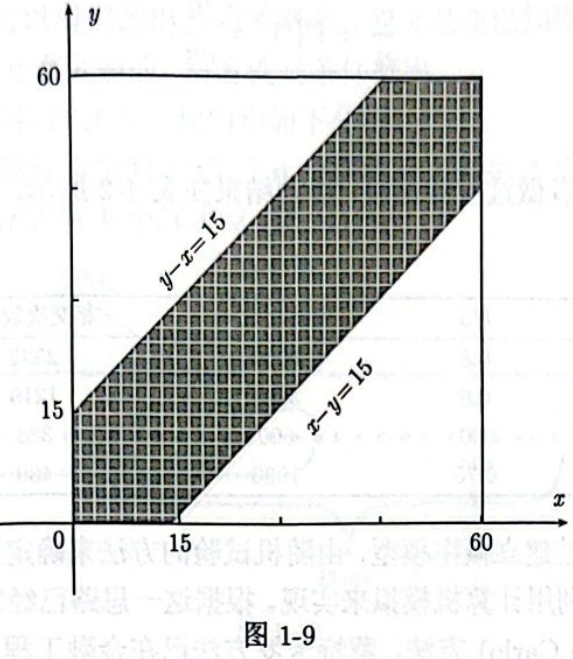
\includegraphics[scale = 0.4]{figures/figure1-9.png}
		\end{figure}
	\end{frame}
	
	\begin{frame}
		有几何计算可知
		\[
		P(A) = (60 ^ 2 - 45 ^ 2) / 60 ^ 2 = 7 / 16
		\]
	\end{frame}
	
	\begin{frame}
		\frametitle{条件概率}
		定义 1.3 设A,B为两个随机事件,且$P(B) > 0$,称
		\[
		P(A|B) = \frac{P(A \cap B)}{P(B)}
		\]
		为在事件B发生的条件下,事件A发生的概率。
		
		条件概率$P(\cdot | B)$满足概率的三条性质
		
		\begin{enumerate}
			\item 非负性 对于任意事件A,$P(A|B) \geq 0$;
			\item 规范性 $P(\Omega | B) = 1$;
			
			\[
			P(\Omega | B) = P( \Omega \cap B) / P(B) = P(B) / P(B) = 1
			\]
			\item 可列可加性 若$A_1, A_2, \dots$两两互不相容,则
			\[
			P(\cup_{i = 1}^{\infty}A_i | B) = \sum_{i = 1}^{\infty}P(A_i |B) 
			\]
		\end{enumerate}
	\end{frame}
	
	\begin{frame}
		\begin{itemize}
			\item
			\begin{align}
			P(\cup_{i = 1}^{\infty}A_i | B) &= \frac{P(\cup_{i = 1}^{\infty}A_i \cap B)}{P(B)} \\ 
			&= \frac{P(\cup_{i = 1}^{\infty}(A_i \cap B))}{P(B)} \qquad(\text{分配率})\\
			&= \sum_{i = 1}^{\infty} \frac{P(A_i \cap B)}{P(B)} \\
			&\qquad(A_i\text{两两互斥则}(A_i \cap B)\text{两两互斥})\nonumber \\
			& = \sum_{i = 1}^{\infty}P(A_i |B)
			\end{align}
		\end{itemize}
	\end{frame}
	
	\begin{frame}
		例 1.13 一共10个元件4个次品,6个正品。从中任取两个。已知第一个是正品,求第二个事正品的概率。
		
%		\begin{itemize}
%			\item 事件$A = \{\text{第二个是正品}\}, B = \{\text{第一个是正品}\}$。$P(B) = 6 / 10$。 $P(A\cap B) = P(\text{第一个和第二个都是正品}) = C_6^2 / C_{10}^2 = 1 / 3$。
%			\[
%			P(A|B) = \frac{P(A\cap B)}{P(B)} = 5 / 9
%			\]
%			\item 当第一次抽取的情况已经确定。可以直接考虑第二次抽取。这时一共有9个选择,其中正品5个。所以在第一次抽取正品的前提下第二次抽取正品的概率是5/9.
%		\end{itemize}
	\end{frame}
	
	\begin{frame}
		例 1.13 一共10个元件4个次品,6个正品。从中任取两个。已知第一个是正品,求第二个事正品的概率。
		
		\begin{itemize}
			\item 事件$A = \{\text{第二个是正品}\}, B = \{\text{第一个是正品}\}$。$P(B) = 6 / 10$。 $P(A\cap B) = P(\text{第一个和第二个都是正品}) = C_6^2 / C_{10}^2 = 1 / 3$。
			\[
			P(A|B) = \frac{P(A\cap B)}{P(B)} = 5 / 9
			\]
			\item 当第一次抽取的情况已经确定。可以直接考虑第二次抽取。这时一共有9个选择,其中正品5个。所以在第一次抽取正品的前提下第二次抽取正品的概率是5/9.
		\end{itemize}
	\end{frame}
	
	\begin{frame}
		在条件概率有定义的条件下,$P(B)>0$,
		\[
		P(A\cap B)= P(B) P(A|B)
		\]
		被称为乘法公式。
	\end{frame}
		
	\begin{frame}
		例 1.15 某种光学透镜,第一次落下时被打破的概率是1/2。如果第一次下落未打破,第二次下落打破的概率是7/10。如果前两次没有打破,第三次下落打破的概率是9/10.求三次下落未打破的概率。
		
		%		首先定义事件$A_i$代表第$i = 1, 2, 3$次未打破。B为三次都未打破。这样$B =A_1 \cap A_2 \cap A_3$.
		%		
		%		\begin{align}
			%			P(B) &= P( A_1 \cap A_2 \cap A_3) \\
			%			&= P(A_3 | A_1 \cap A_2) P( A_1 \cap A_2) \\
			%			&= P(A_3 | A_1 \cap A_2) P( A_2 | A_1) P(A_1) \label{e1}
			%		\end{align}
		%		$P(A_1) = 1 - P(\text{第一次打破}) = 1 - 1 / 2 = 1 / 2$。
		%		
		%		$P(A_2|A_1) = 1 - 7 / 10$
		%		
		%		$P(A_3|A_2 \cap A_1) = 1 - 9 / 10$
		%		带入(\ref{e1})得到$P(B) = 3 / 200$
	\end{frame}
	
	\begin{frame}
		例 1.15 某种光学透镜,第一次落下时被打破的概率是1/2。如果第一次下落未打破,第二次下落打破的概率是7/10。如果前两次没有打破,第三次下落打破的概率是9/10.求三次下落未打破的概率。
		
		首先定义事件$A_i$代表第$i = 1, 2, 3$次未打破。B为三次都未打破。这样$B =A_1 \cap A_2 \cap A_3$.
		
		\begin{align}
			P(B) &= P( A_1 \cap A_2 \cap A_3) \\
			&= P(A_3 | A_1 \cap A_2) P( A_1 \cap A_2) \\
			&= P(A_3 | A_1 \cap A_2) P( A_2 | A_1) P(A_1) \label{e1}
		\end{align}
		$P(A_1) = 1 - P(\text{第一次打破}) = 1 - 1 / 2 = 1 / 2$。
		
		$P(A_2|A_1) = 1 - 7 / 10$
		
		$P(A_3|A_2 \cap A_1) = 1 - 9 / 10$
		带入(\ref{e1})得到$P(B) = 3 / 200$
	\end{frame}
	
	\begin{frame}
		例 1.16 n把钥匙中只有一把可以打开门。不重复依次尝试各个钥匙,求第k次才打开门的概率($k \leq n$).
		
%		令$A_i = \{\text{第i次不能打开门}\}$。则$B = \{k\text{次才能打开门}\} = A_1 \cap A_2 \cap A_3 \cap \dots \bar{A_k}$
%		\begin{align}
%			P(B) & = P(A_1 \cap A_2 \cap A_3 \cap \dots \bar{A_k}) \\
%			& = P(A_1) P(A_2 | A_1) \dots P(A_k | A_{k - 1} \cap A_{K - 2} \cap \dots A_1) \\
%			& = \frac{n - 1}{n} \frac{n - 2}{n - 1} \cdots \frac{1}{n - (k - 1)} \\
%			& = \frac{1}{n}
%		\end{align}
	\end{frame}
	
	\begin{frame}
		例 1.16 n把钥匙中只有一把可以打开门。不重复依次尝试各个钥匙,求第k次才打开门的概率($k \leq n$).
		
		令$A_i = \{\text{第i次不能打开门}\}$。则$B = \{k\text{次才能打开门}\} = A_1 \cap A_2 \cap A_3 \cap \dots \bar{A_k}$
		\begin{align}
			P(B) & = P(A_1 \cap A_2 \cap A_3 \cap \dots \bar{A_k}) \\
			& = P(A_1) P(A_2 | A_1) \dots P(A_k | A_{k - 1} \cap A_{K - 2} \cap \dots A_1) \\
			& = \frac{n - 1}{n} \frac{n - 2}{n - 1} \cdots \frac{1}{n - (k - 1)} \\
			& = \frac{1}{n}
		\end{align}
	\end{frame}
	
	\begin{frame}
		定义 1.4 若$n$个事件$A_i, i = 1, \dots, n$满足
		\begin{itemize}
			\item \new{任何$A_i$不是空集}
			\item $A_i, A_j, 1 \leq i \neq j \leq n$两两互不相容
			\item $\cup_{i = 1}^nA_i = \Omega$
		\end{itemize}
		则称$A_i, i = 1, \dots, n$为样本空间$\Omega$的一个\textbf{划分}或者\textbf{完备事件组}。
		若事件$A_i, i = 1, \dots, n$为划分,则在每次随机试验中必有且仅有一个$A_i$发生。
		
		定理 1.1(全概率公式)设$A_i, i = 1, \dots, n$是一个划分,则对任何事件$B$有
		\[
		P(B) = \sum_{i = 1}^{n}P(A_i)P(B | A_i)
		\]
	\end{frame}
	\begin{frame}
		首先观察等式右边$P(A_i)P(B | A_i) = P(B \cap A_i)$。继续观察发现等号右边是求和。联系到性质(2),如果$B = \cup_{i = 1}^n (B \cap A_i)$,且$B \cap A_i$两两互斥,则定理得证。因为$A_i, i = 1, \dots, n$是一个划分,所以$\cup_{i = 1}^nA_i = \Omega$。这样$B \cap \Omega = B \cap (\cup_{i = 1}^{n}A_i)$。由分配律可得$B = \cup_{i = 1}^n (B \cap A_i)$。
		
		\vspace*{1cm}
		证明:$B = B \cap \Omega = B\cap (\cup_{i = 1}^{n}A_i) = \cup_{i = 1}^n (B \cap A_i)$.因为$A_i, A_j$对所有$i \neq j$两两互斥,则$B \cap A_i, B \cap A_j$两两互斥。由此
		\[
		P(B) = P(\cup_{i = 1}^n (B \cap A_i)) = \sum_{i = 1}^{n} P(B \cap A_i) = \sum_{i = 1}^{n}P(A_i)P(B | A_i) 
		\]
	\end{frame}
	
	\begin{frame}
		例 1.17 甲袋中有5个球(3红2白),乙袋中有8个球(4红4白)。先从甲袋中取2个球放入乙袋。再从乙袋中取出一个球。请问乙袋中取出白球的概率。
		
%		由于从乙袋中取出白球的情况取决于放入乙袋是什么样的球。所以分步考虑。
%		设$A_1: \text{甲袋中取出两个白球}, A_2: \text{甲袋中取出两个红球}, A_3: \text{甲袋中取出1个红球}$。则
%		\begin{align}
%			P(A_1) &= 1 / C_5^2 \\
%			P(A_2) &= C_3^2 / C_5^2 \\
%			P(A_3) &= C_3^1 C_2^1 / C_5^2
%		\end{align}
%		然后
%		\begin{align}
%			P(B | A_1) &= 6 / 10 \\
%			P(B | A_2) &= 4 / 10 \\
%			P(B | A_3) &= 5 / 10
%		\end{align}
%		由此可得
%		\[
%		P(B) = \sum_{i = 1}^{3}P(B | A_i)P(A_i) = 48 / 100 
%		\]
	\end{frame}
	
	\begin{frame}
		例 1.17 甲袋中有5个球(3红2白),乙袋中有8个球(4红4白)。先从甲袋中取2个球放入乙袋。再从乙袋中取出一个球。请问乙袋中取出白球的概率。
		
		由于从乙袋中取出白球的情况取决于放入乙袋是什么样的球。所以分步考虑。
		设$A_1: \text{甲袋中取出两个白球}, A_2: \text{甲袋中取出两个红球}, A_3: \text{甲袋中取出1个红球}$。则
		\begin{align}
			P(A_1) &= 1 / C_5^2 \\
			P(A_2) &= C_3^2 / C_5^2 \\
			P(A_3) &= C_3^1 C_2^1 / C_5^2
		\end{align}
		然后
		\begin{align}
			P(B | A_1) &= 6 / 10 \\
			P(B | A_2) &= 4 / 10 \\
			P(B | A_3) &= 5 / 10
		\end{align}
		由此可得
		\[
		P(B) = \sum_{i = 1}^{3}P(B | A_i)P(A_i) = 48 / 100 
		\]
	\end{frame}
	
	\begin{frame}
		例 1.18 设甲袋有 $N-1$ 只白球和 1 只黑球, 乙袋中有 $N$ 只白球.若每次从甲、乙户 袋中各取一球交换, 记 $A_{k}$ 为经过 $k$ 次交换后黑球仍在甲袋中, 证明:
		
		\begin{align*}
			&P\left(A_{k+1}\right)\\
			&=\frac{1}{N}+\left(1-\frac{2}{N}\right) P\left(A_{k}\right), \quad k=1,2, \cdots
		\end{align*}
	\end{frame}
	
	\begin{frame}
		证明 $A_{k}$ 表示 $k$ 次交换后黑球仍在甲袋, 因此, $A_{k}$ 发生时, 甲袋有 $N-1$ 只白球 1 只黑球, 此后若 $A_{k+1}$ 发生, 等价于从甲袋取出白球; $\bar{A}_{k}$ 发生时, 乙袋有 $N-1$ 只白球 1 只黑球, 此后若 $A_{k+1}$ 发生, 等价于从乙袋取出黑球, 因此
		
		$$
		P\left(A_{k+1} \mid A_{k}\right)=\frac{N-1}{N}, P\left(A_{k+1} \mid \bar{A}_{k}\right)=\frac{1}{N} \text { . }
		$$
		
		由全概率公式,
		
		$$
		\begin{aligned}
			P\left(A_{k+1}\right) & =P\left(A_{k}\right) P\left(A_{k+1} \mid A_{k}\right)+P\left(\bar{A}_{k}\right) P\left(A_{k+1} \mid \bar{A}_{k}\right) \\
			& =P\left(A_{k}\right) \frac{N-1}{N}+\left[1-P\left(A_{k}\right)\right] \frac{1}{N} \\
			& =\frac{1}{N}+\left(1-\frac{2}{N}\right) P\left(A_{k}\right) .
		\end{aligned}
		$$
	\end{frame}
		
	\begin{frame}
		定理 1.2(\textbf{贝叶斯公式}) 设$\{A_i, i = 1, 2, \dots, n\}$为划分,则对事件$B$有
		\[
		P(A_i | B) = \frac{P(A_i)P(B | A_i)}{\sum_{k = 1}^{n}P(A_k)P(B | A_k)}
		\]
		
	\end{frame}
	
	\begin{frame}
		观察等式左边,$P(A_i | B) = P(A_i \cap B) / P(B)$。而等式右边分子等于$P(A_i \cap B)$。如此只需证明分母等于$P(B)$。由全概率公式可得出$P(B) = \sum_{k = 1}^{n}P(A_k)P(B | A_k)$。
		证明:
		\[
		P(A_i | B) = \frac{P(A_i \cap B)}{P(B)} = \frac{P(A_i)P(B | A_i)}{\sum_{k = 1}^{n}P(A_k)P(B | A_k)}
		\]
	\end{frame}
	
	\begin{frame}
		例 1.17 甲袋中有5个球(3红2白),乙袋中有8个球(4红4白)。先从甲袋中取2个球放入乙袋。再从乙袋中取出一个球。
		
		例 1.19 延续例 1.17:已知最后从乙袋中取出白球,问从甲袋中放入乙袋的2球都是红球的概率。
	\end{frame}
	
	\begin{frame}
		\[
		P(A_2 | B) = \frac{P(A_2 \cap B)}{\sum_{i = 1}^{3}P(A_i)P(B | A_i)} = \frac{12}{48}
		\]
	\end{frame}
	
	\begin{frame}
		例 1.20 一批产品中有96\%是合格品。现有一种简化的检查方法,它把合格品判为合格品的概率是0.98,把不合格品误判为合格品的概率为0.05。任取一件产品。计算
		\begin{enumerate}
			\item 判定结果为合格品的概率。
			\item 给定判定结果为合格品,产品确实合格的概率。
		\end{enumerate}
	\end{frame}
	
	\begin{frame}
		首先定义事件。$A: \text{取到合格品}, B: \text{判定结果为合格品}$。这样两个问题分别计算$P(B)$与$P(A | B)$。整理题目给出的信息可知
		\begin{align}
			P(A) &= 0.96 \\
			P(\bar{A}) &= 1 - 0.96 = 0.04 \\
			P(B | A) &= 0.98 \\
			P(B | \bar{A}) &= 0.05
		\end{align}
		由全概率公式可得
		\[
		P(B) = P(A) P(B | A) + P(\bar{A}) P(B | \bar{A}) = 0.9428
		\]
		由条件概率定义可得
		\[
		P(A | B) = \frac{P(A)P(B | A)}{P(B)} = 0.96 \times 0.98 / 0.9428 =0.9979
		\]
	\end{frame}
		
	\begin{frame}
		例 1.21某学生接连参加同一课程的两次考试,第一次及格概率为$p$。若第一次及格则第二次及格的概率也为$p$;若第一次不及格则第二次及格概率为$p / 2$。请计算
		\begin{enumerate}
			\item 至少一次及格概率。
			\item 在第二次及格的条件下,第一次及格的概率。
		\end{enumerate}
	\end{frame}
	
	\begin{frame}
		首先定义事件$A_i: \text{第i次考试及格}, i = 1, 2$。至少一次及格的对立事件是两次都不及格即$A_1 \cap A_2$。可由条件概率公式求得。若第二次及格,第一次及格的概率为条件概率$P(A_1 | A_2)$。
		
		\vspace*{1cm}
		整理题目信息可得$P(A_1) = p, P(A_2 | A_1) = p, P(A_2 | \bar{A_1}) = p /2 $
		\begin{enumerate}
			\item \begin{align}
				P(A_1 \cup A_2) & = 1 - P(\overline{A_1 \cup A_2}) \\
				& = 1 - P(\bar{A_1} \cap \bar{A_2}) \\
				& = 1 - P(\bar{A_2} | \bar{A_1})P(\bar{A_1}) \\
				& = 1 - (1 - P(A_2 | \bar{A_1}))P(\bar{A_1})  \\ 
				& = 1 - (1 - P(A_2 | \bar{A_1}))(1 - P(A_1)) \\
				& = 1 - (1 - P / 2)(1 - p) \\
				& = \frac{3}{2}p - \frac{p ^ 2}{2}
			\end{align}
		\end{enumerate}
	\end{frame}
	
	\begin{frame}
		\begin{enumerate}\setcounter{enumi}{1}
			\item \begin{align}
				P(A_1 | A_2) & = P(A_1 \cap A_2) / P(A_2) \\
				& = \frac{P(A_1)P(A_2 |A_1)}{P(A_1)P(A_2 |A_1) + P(\bar{A_1})P(A_2 |\bar{A_1})} \\
				& = \frac{p \times p}{p \times p + p / 2 \times(1 - p)} \\
				& = \frac{2p}{p + 1}
			\end{align}
		\end{enumerate}
	\end{frame}
	
	\begin{frame}
		\frametitle{独立性}
		定义 1.5 设$A, B$是两个随机事件。若满足等式
		\[
		P(A \cap B) = P(A) P(B)
		\]
		则称$A, B$相互独立,简称$A, B$独立。
		
		\vspace{1cm}
		例 1.22 袋中有a只黑球,b只白球。每次从中取出1球。令
		\begin{align}
			A & = \{\text{第一次取出白球}\} \\
			B & = \{\text{第二次取出白球}\}
		\end{align}
		分别对放回与不放回情形讨论$A, B$的是否独立。
	\end{frame}
	
	\begin{frame}
		\begin{itemize}
			\item 不放回:
			
			$P(A) = \frac{b}{a + b}, P(B) = \frac{b}{a + b}$
			\[
			P(A \cap B) = C_b^2 / C_{a + b}^2 = \frac{b(b - 1)}{(a + b)(a + b -1)}
			\]
			可知$P(A \cap B) \neq P(A) P(B)$ A与B不独立。
			
			\item 放回:
			
			$P(A) = \frac{b}{a + b}, P(B) = \frac{b}{a + b}, P(A \cap B) = \frac{b \times b}{(a + b)(a + b)}$。可知$P(A \cap B) = P(A)P(B)$,则A,B独立。
			
		\end{itemize}
	\end{frame}
	
	\begin{frame}
		定理 1.3 若随机事件A、B独立,则$\bar{A} \text{与} B$,$A \text{与} \bar{B}$, $\bar{A} \text{与} \bar{B}$也相互独立。
		
		只需按定义证明$P(\bar{A} \cap B) = P(\bar{A}) P(B)$
		
		证:因为A,B独立,$P(A \cap B) = P(A) P(B)$。
		\begin{align}
			P(\bar{A} \cap B) & = P(B - A) = P(B) - P(A \cap B) \\
			& = P(B) - P(A)P(B) \\
			& = P(B)(1 - P(A)) \\
			& = P(B)P(\bar{A})
		\end{align}
		同理可得其余事件对相互独立。
	\end{frame}
	
	\begin{frame}
		如果$n$个事件$A_1, A_2, \dots, A_n$独立则需以下条件成立:
		\begin{align}
			\begin{cases}
				& P(A_i \cap A_j) = P(A_i)P(A_j), \quad 1 \leq i < j \leq n \\
				& P(A_i \cap A_j \cap A_k ) =  P(A_i)P(A_j)P(A_k), \quad 1 \leq i < j < k \leq n\\
				& \dots \\
				& P(A_{i1} \cap A_{i2} \cap \dots \cap A_{im}) = P(A_{i1})P(A_{i2})\cdots P(A_{im}) \\
				& \dots \\
				& P(A_1 \cap A_2 \cap A_3 \cap \cdots \cap A_n) = P(A_1)P(A_2)\cdots P(A_n)
			\end{cases}\nonumber
		\end{align}
	\end{frame}
	
	\begin{frame}
		定理1.4 设事件$A_1, A_2, \dots, A_n$相互独立,将其分为没有公共事件的$k$组。每个组任意做事件(集合)运算,得到一个新事件,则这$k$个新事件相互独立。n个独立事件的加法定理如下:
		\[
		P(\cup_{i = 1}^{n}A_i) = 1 - \prod_{i = 1}^{n} P(\bar{A_i})
		\]
		
%		要把$\cup_{i = 1}^{n}A_i$与$\bar{A_i}$建立联系考虑$\cup_{i = 1}^{n}A_i$的补集。
%		
%		\begin{align}
%			P(\cup_{i = 1}^{n}A_i) &= 1 - P(\overline{\cup_{i = 1}^{n}A_i}) \\
%			& = 1 - P( \cap_{i = 1}^n \bar{A_i}) \\
%			& = 1 - \prod_{i = 1}^{n}P(\bar{A_i})
%		\end{align}
	\end{frame}
	
	\begin{frame}
		定理1.4 设事件$A_1, A_2, \dots, A_n$相互独立,将其分为没有公共事件的$k$组。每个组任意做事件(集合)运算,得到一个新事件,则这$k$个新事件相互独立。n个独立事件的加法定理如下:
		\[
		P(\cup_{i = 1}^{n}A_i) = 1 - \prod_{i = 1}^{n} P(\bar{A_i})
		\]
		
		要把$\cup_{i = 1}^{n}A_i$与$\bar{A_i}$建立联系考虑$\cup_{i = 1}^{n}A_i$的补集。
		
		\begin{align}
			P(\cup_{i = 1}^{n}A_i) &= 1 - P(\overline{\cup_{i = 1}^{n}A_i}) \\
			& = 1 - P( \cap_{i = 1}^n \bar{A_i}) \\
			& = 1 - \prod_{i = 1}^{n}P(\bar{A_i})
		\end{align}
	\end{frame}
	
	\begin{frame}
		\textbf{小概率事件原理}
		
		 独立重复试验中事件$A$发生的概率为$p$。当试验重复次数$n\rightarrow \infty$,$P(\text{A至少发生一次}) \rightarrow 1$。
		 
		 \vspace*{1cm}
		 首先定义事件$A_i: \text{第i次试验时A不发生。}$
		 \begin{align}
		 	P(\text{A至少发生一次}) & = 1 - P(\text{A不发生}) \\
		 	& = 1 - P(\bar{A_1} \cap \bar{A_2} \cap \cdots \cap \bar{A_n}) \\
		 	& = 1 - \prod_{i = 1}^{n} P(\bar{A_i}) \\
		 	& = 1 - \prod_{i = 1}^{n}(1 - P(A_i)) \\
		 	& = 1 - (1 - p)^n \\
		 	& \rightarrow 1 - 0 \rightarrow 1 
		 \end{align}
	\end{frame}
	
	\begin{frame}
		例 1.24 甲乙丙三人对同一目标各自进行一次射击。假设三次射击为独立试验,且三人命中概率分别为0.6、0.7、0.8。请计算
		\begin{enumerate}
			\item 目标至少被一人命中概率。
			\item 恰有一人命中概率。
		\end{enumerate}
	\end{frame}
	
	\begin{frame}
		用$A_1, A_2, A_3$分别表示甲、乙、丙三人命中目标。至少一人命中的对立事件是三人全部没有命中,即$\bar{A_1} \cap \bar{A_2} \cap \bar{A_3}$。恰有一人命中为事件$(A_1 \cap \bar{A_2} \cap \bar{A_3}) \cup (\bar{A_1} \cap A_2 \cap \bar{A_3}) \cup (\bar{A_1} \cap \bar{A_2} \cap A_3)$
		\begin{enumerate}
			\item $P(\{\text{至少一人命中}\}) = 1 - P(\bar{A_1} \cap \bar{A_2} \cap \bar{A_3}) = 1 - ( 1 - 0.6)(1 - 0.7)(1 - 0.8)$
			\item \begin{align}
				&P(\text{仅有一次命中}) \\
				& = P((A_1 \cap \bar{A_2} \cap \bar{A_3}) \cup (\bar{A_1} \cap A_2 \cap \bar{A_3}) \cup (\bar{A_1} \cap \bar{A_2} \cap A_3)) \\ 
				& = P(A_1 \cap \bar{A_2} \cap \bar{A_3}) + P(\bar{A_1} \cap A_2 \cap \bar{A_3}) + P(\bar{A_1} \cap \bar{A_2} \cap A_3) \\
				& = P(A_1) P(\bar{A_2}) P(\bar{A_3}) + P(\bar{A_1}) P(A_2) P(\bar{A_3}) + P(\bar{A_1}) P(\bar{A_2}) P(A_3) \\
				& = 0.6 \times 0.3 \times 0.2 + 0.4 \times 0.7 \times 0.2 + 0.4 \times 0.3 \times 0.8
			\end{align}
		\end{enumerate}
	\end{frame}
	
	\begin{frame}
		一个元件或者系统的\textbf{可靠性}指其正常工作的概率。
		
		$A_i: \text{元件i正常工作}$, $B_j: \text{系统j正常工作}$。假设每个元件独立工作。$P(A_i) = p_i$。
		\begin{itemize}
			\item 串联方式构成的系统
			\begin{figure}[H]
				\centering
				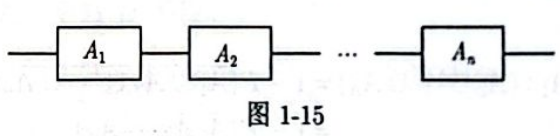
\includegraphics[scale = 0.3]{figures/figure1-15.png}
			\end{figure}
			$P(B_1) = P(A_1 \cap \dots \cap A_n) = \prod_{i = 1}^{n}P(A_i)$
			\item 并联方式构成的系统
			\begin{figure}[H]
			\centering
			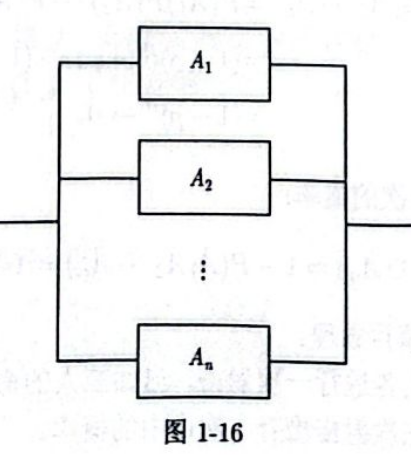
\includegraphics[scale = 0.2]{figures/figure1-16.png}
			\end{figure}
			$P(B_2) = P(\cup_{i = 1}^{n}A_i) = 1 - P(\cap_{i = 1}^n\bar{A_i}) = 1 - \prod_{i = 1}^{n}(1 - p_i)$
		\end{itemize}
	\end{frame}
	
	\begin{frame}
		例 1.25 如图1-17所示系统由$2n$个独立工作元件构成,每个元件可靠性为$0 < p < 1$。求解则系统可靠性。
		\begin{figure}[H]
			\centering
			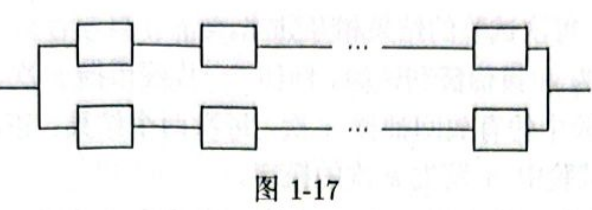
\includegraphics[scale = 0.3]{figures/figure1-17.png}
		\end{figure}
	\end{frame}
	
	\begin{frame}
		由于系统上下两部分相对独立则可将整个系统分为两个串联子系统。每个子系统正常工作概率为$p^n$。
		\begin{align}
			P(\text{整个系统工作}) & = P(\text{上下子系统至少一个工作}) \\
			& = 1 - P(\text{两个子系统都不工作}) \\
			& = 1 - (1 - p^n)^2\\
			& = 2p^n - p^{2n}
		\end{align}
	\end{frame}
	
	\begin{frame}
		例 1.25 如下图所示系统由5个独立工作的元件构成。假设每个元件可靠性为$p$。请计算整个系统可靠性。
		\begin{figure}
			\centering
			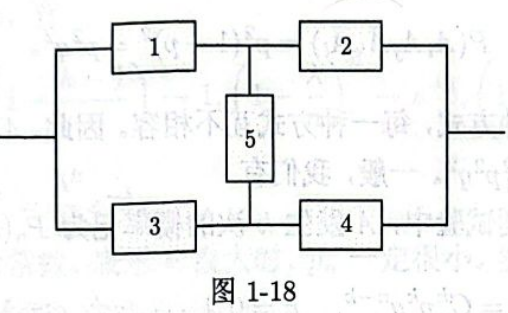
\includegraphics[scale = 0.3]{figures/figure1-18.png}
		\end{figure}
	\end{frame}
	
	\begin{frame}
		设$A_i, i = 1, 2, 3, 4, 5,$表示第i个元件工作, $B:\text{整个系统工作}$。可由任意元件是否工作为出发点。解中以元件5为例。
		\begin{align}
			P(B | A_5) & = P((A_1 \cup A_3) \cap (A_2 \cup A_4)) \\ 
			& = P(A_1 \cup A_3) P(A_2 \cup A_4) \\
			& = (1 - (1 - p) ^ 2)(1 - (1 - p) ^ 2) \\
			& = (2p - p ^ 2) ^ 2
		\end{align}
		元件5不工作的情况符合例 1.25中情形,此时$n = 2$,因此$P(B | \bar{A_5}) = 2p^2 - p^4$。
		
		由全概率公式
		\begin{align}
			P(B) & = P(A_5)P(B | A_5) + P(\overline{A_5})P(B | \overline{A_5}) \\
			& = p(2p - p ^ 2) ^ 2 + (1 - p)(2p^2 - p^4)
		\end{align}
	\end{frame}
	
	\begin{frame}
		\frametitle{独立重复试验}
		\textbf{n重伯努利试验}是一类重要的独立重复试验,其具有如下特点:
		\begin{itemize}
			\item 每次试验只有两种结果$A$与$\bar{A}$,$P(A) = p, P(\bar{A}) = 1 - p = q$。
			\item 试验重复$n$次,每次试验的结果独立。
		\end{itemize}
	\end{frame}
	
	\begin{frame}
		定理 1.5 $n$重伯努利试验中,$A$发生$k$次的概率记为$P_n(k)$,则
		\[
		P_n(k) = C_n^k p^k(1 - p)^{n - k}, k = 0, 1, \dots, n
		\]
		
		注意:$\sum_{k = 0}^{n}P_n(k) = \sum_{k = 1}^{n}C_n^k p^k(1 - p)^{n - k} = (p + 1 - p) ^ n = 1$
	\end{frame}
	
	\begin{frame}
		例 1.27 一大批样品的次品率是0.1。现从中随机取出20件。求:
		\begin{enumerate}
			\item 取到两件次品的概率。
			\item 至少取到两件次品的概率。
		\end{enumerate}
			注释:因为样品量大,取出20件样品的过程可以近似认为是从中独立重复取了20次样品。
	\end{frame}
	
	\begin{frame}
		$A:\text{此次取出次品}$。$p = P(A) = 0.1$。取$k$件次品的概率:$P_{20}(k) = C_{20}^k 0.1 ^ k (1 - 0.1) ^ {20 - k}$
		\begin{enumerate}
			\item $P_{20}(2) = C_{20}^2 0.1 ^ 2 (1 - 0.1) ^ {20 - 2} = 0.2852$
			\item $P(\text{至少取得两件次品}) = 1 - P_{20}(0) - P_{20}(1) = 1 - 0.9^{20} - C_{20}^1 \times 0.1 \times 0.9 ^ {19} = 0.6083$
		\end{enumerate}
	\end{frame}
	
	\begin{frame}
		定理 1.6(泊松定理) 设$n$为正整数,$p_n \in [0, 1], \lambda = np_n$为常数。则对任意正整数$k$有
		\[
		\lim_{n \rightarrow \infty} C_n^k p_n^k(1 - p_n)^{n - k} = \frac{\lambda ^ k}{k!}\exp ^{ -\lambda}
		\] 
	\end{frame}
	
	\begin{frame}
		证:$p_n = \lambda / n$,则
		\begin{align}
			&C_n^k p_n^k(1 - p_n)^{n - k} \\
			& = \frac{n(n - 1)\cdots(n - k + 1)}{k!}(\frac{\lambda}{n}) ^ k ( 1 - \lambda / n) ^ {n - k} \\
			& = \frac{\lambda^k}{k!}\left[1\times (1 - \frac{1}{n}) \cdots( 1 - \frac{k - 1}{n})\right](1 - \lambda / n) ^ n( 1 - \lambda / n) ^ {-k} \\
		\end{align}
		对于任意固定的$k$,当$n \rightarrow \infty$
		
		$1\times (1 - \frac{1}{n}) \cdots( 1 - \frac{k - 1}{n}) \rightarrow 1$
		
		$(1 - \lambda / n) ^ n \rightarrow \exp ^ {-\lambda}$
		
		$( 1 - \lambda / n) ^ {-k} \rightarrow 1$
		这样$\lim_{n \rightarrow \infty} C_n^k p_n^k(1 - p_n)^{n - k} = \frac{\lambda ^ k}{k!}\exp ^{ -\lambda}$
	\end{frame}
	
	\begin{frame}
		在实际应用中,$n$充分大,$p_n$充分小,则可令$\lambda = np_n$,此时
		\[
		C_n^k p_n^k(1 - p_n)^{n - k} \approx \frac{\lambda ^ k}{k!}\exp ^{ -\lambda}
		\]
		
		例 1.29 做$n = 800$次独立重复试验,$P(A) = p = 0.002$。利用泊松近似公式计算$A$发生不超过3次的概率。
		
		\vspace*{1cm}
		$\lambda = np_n = 800 \times 0.002 = 1.6$,$A$发生$k$次的概率
		\[
		P_{800}(k) = C_{800}^K0.002^K\times(1 - 0.002)^{800 - k} \approx \frac{1.6^k}{k!}\exp ^{-1.6}
		\]
		则所求概率
		\[
		P(\text{A发生不超过3次}) = \sum_{k = 0}^{3}P_{800}(k) \approx \sum_{k = 0}^{3}\frac{1.6^k}{k!}\exp ^{-1.6} = 0.9212
		\]
	\end{frame}
\end{document}